%公式的上下间距
\setlength{\abovedisplayskip}{0pt}
\setlength{\belowdisplayskip}{0pt}

\subsection{研究方法与技术路线}

本项目将采用理论推导结合数值验证的方法进行研究,
首先,研究哈密顿原理伽辽金弱形式中拉格朗日乘子型虚位移本质边界条件施加方案,并验证相对应的弱形式与欧拉--拉格朗日方程之间的等价性。
其次,基于再生核无网格近似,通过对相对应的离散控制方程进行局部截断误差分析,确定时空混合离散再生核无网格近似阶次,以缓解数值色散问题。
随后,依托再生光滑梯度理论框架,构建适用于时空混合离散的变分一致型伽辽金无网格数值积分方案。
最后,将所提再生核近似方案与变分一致型数值积分方案引入拉格朗日乘子型时空混合离散伽辽金弱形式,建立适用于任意节点分布的稳定时空混合离散伽辽金无网格法。
具体的技术路线图如下所示。

\begin{figure}[!h]
    \centering 
    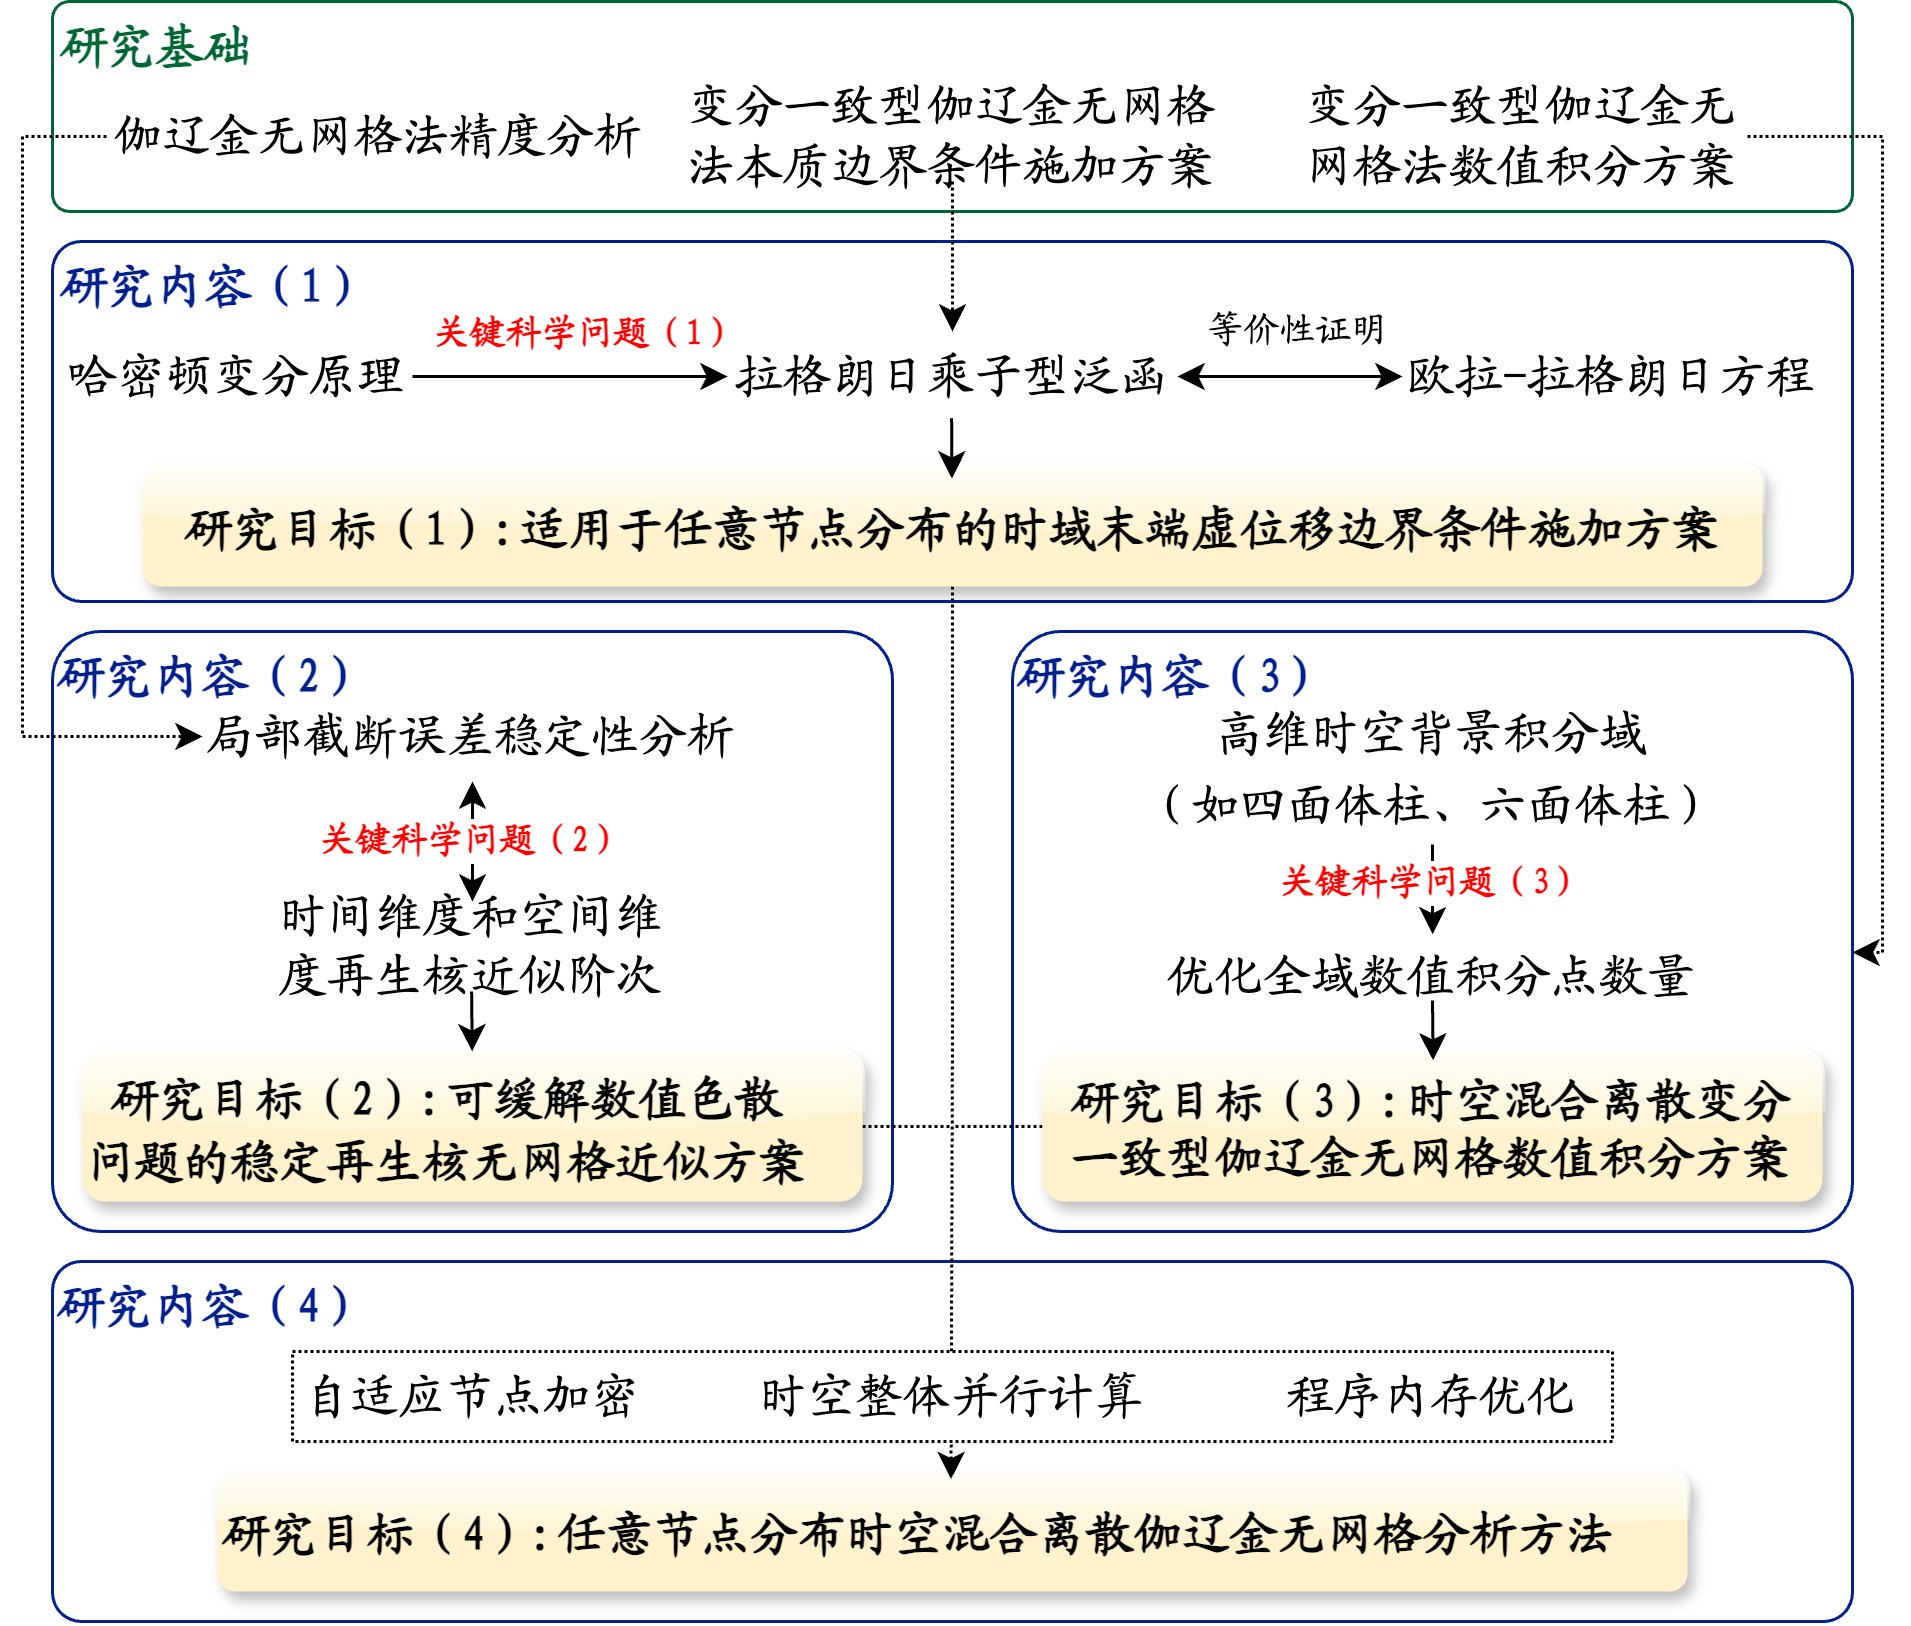
\includegraphics[width=\textwidth]{figures/roadmap.png}
    \caption{技术路线图}
    \label{fg:roadmap}
\end{figure}

\subsection{研究方案}

\subsubsection*{\bfseries (1)适用于任意节点分布的时域末端虚位移本质边界条件施加方案}
首先,查阅基于哈密顿变分原理时空混合离散有限元法的相关文献,确定虚位移本质边界条件的几种可能性。
将不同虚位移边界的方法进行数值实现,对比计算结果的稳定性和精度。
确定稳定性最优情况下的虚位移空间$\tilde V_h$,相对应的变分问题为:
\begin{equation}
    \text{find} \; u_h \in V_h, \quad a(u_h, \delta u_h) = f(\delta u_h), \quad \forall \delta u_h \in \tilde V_h
    \label{eq:1}
\end{equation}
其中,$V_h$为位移空间,$a:V\times V \rightarrow \mathbb R$为双线性算子,$f:V\rightarrow \mathbb R$为线性算子。

随后,将式\eqref{eq:1}中的虚位移$\delta u_h$作为拉格朗日乘子,设计全新拉格朗日乘子型能量泛函:
\begin{equation}
    \text{find} \; u_h \in V_h,\; p_h \in \tilde V_h, \quad
    \left \{
    \begin{split} 
        -a(u_h, \delta u_h) + a(p_h, \delta u_h) = 0,\quad &\forall \delta u_h \in V_h \\
        a(u_h, \delta p_h) = f(\delta p_h),\quad &\forall \delta p_h \in \tilde V_h
    \end{split}
    \right .
    \label{eq:2}
\end{equation}
从上式可以看出,原本式\eqref{eq:1}中的变分问题作为约束条件施加在拉格朗日乘子型伽辽金问题的弱形式中,需进一步在验证两者之间的等价性。
当等价性成立,仅需要采用常规方法对$p_h$施加本质边界条件,即可实现式\eqref{eq:1}中施加虚位移本质边界条件的效果。
同时,引入分部积分公式对式\eqref{eq:2}进行推导,通过修正$u_h$和$p_h$的边界条件,使所提的拉格朗日乘子型伽辽金弱形式满足变分一致性,并证明其与欧拉--拉格朗日方程等价。

最后,采用均布的有限元离散从数值上与传统方法进行对比,验证其计算精度。并用分均布节点离散验证所提方法求解的稳定性。

\subsubsection*{\bfseries (2)可缓解数值色散问题的稳定再生核无网格近似方案}
首先,借鉴von Neumann稳定性分析方法,在拉格朗日型能量泛函所对应的离散控制方程中引入特征解的傅立叶展开式。
同时引入无网格形函数一致性条件,推导均布节点离散下离散控制方程中通用行的局部截断误差估计$\epsilon$,
$\epsilon$应包含时间域节点间距$\Delta t$和空间域节点间距$\Delta x$相关的余项:
\begin{equation}
    \epsilon = O(\Delta t^{n_t}) + O(\Delta x^{n_x})
\end{equation}
其中,$n_t$和$n_x$分别为时间域和空间域的离散阶次。根据截断误差估计,确定空间域离散阶次为$n_x$时,消除数值色散影响所需的时间域离散阶次$n_t$。

随后,在再生核无网格近似的理论框架下,构造相对应阶次的无网格近似基向量$\boldsymbol p^{[n_x,n_t]}$:
\begin{equation}
    \boldsymbol p^{[n_x,n_t]}(x,t) = \left \{1, x, t, x^2, xt, t^2, \dots, x^{n_x}, x^{n_x-1}t, \dots, t^{n_t} \right \}^T
\end{equation}
并根据无网格形函数中矩量矩阵的可逆性,确定核函数影响域在时间维度和空间维度包含节点的个数。

% \begin{figure}[H]
%     \centering
    
% \end{figure}

最后,通过数值验证所提混合离散再生核无网格近似的一致性条件。并代入所提拉格朗日型能量泛函,通过时间域、空间域不同比例节点间距和非均布节点离散测试其是否缓解数值色散问题。

\subsubsection*{\bfseries (3)时空混合离散下变分一致型伽辽金无网格数值积分方案}
首先,根据时空混合离散无网格近似中基向量的元素,推导拉格朗日型伽辽金弱形式的积分约束条件。
引入申请人所提出的再生光滑梯度理论框架,构建满足满足积分约束条件无网格形函数再生光滑梯度,以形函数的一阶时间光滑导数为例,其表达式为:
\begin{equation}
    \tilde \Psi_{I,t}(\boldsymbol x) = \boldsymbol p^{[n_x,n_t - 1]}(\boldsymbol x) \boldsymbol G^{ - 1} \boldsymbol g_{tI}
\end{equation}
其中,$\boldsymbol G$为矩量矩阵,$\boldsymbol g_{tI}$为积分约束条件。再生光滑梯度能自动满足变分一致性条件,适用于相对应阶次的高斯积分方案。

随后,为进一步提升计算效率,将根据再生光滑梯度的一致性条件和数值积分点在单元间的共享特性,优化数值积分点的位置和权重,减少全局数值积分点数量。特别是针对四维空间,拟采用如图 \ref{fg:domain} 所示四面体柱或六面体柱单元作为背景积分域进行数值积分,构建适合时空混合离散再生光滑梯度积分法的数值积分方案。

\begin{figure}[!h]
    \centering 
    \subfloat[四面体柱积分域]{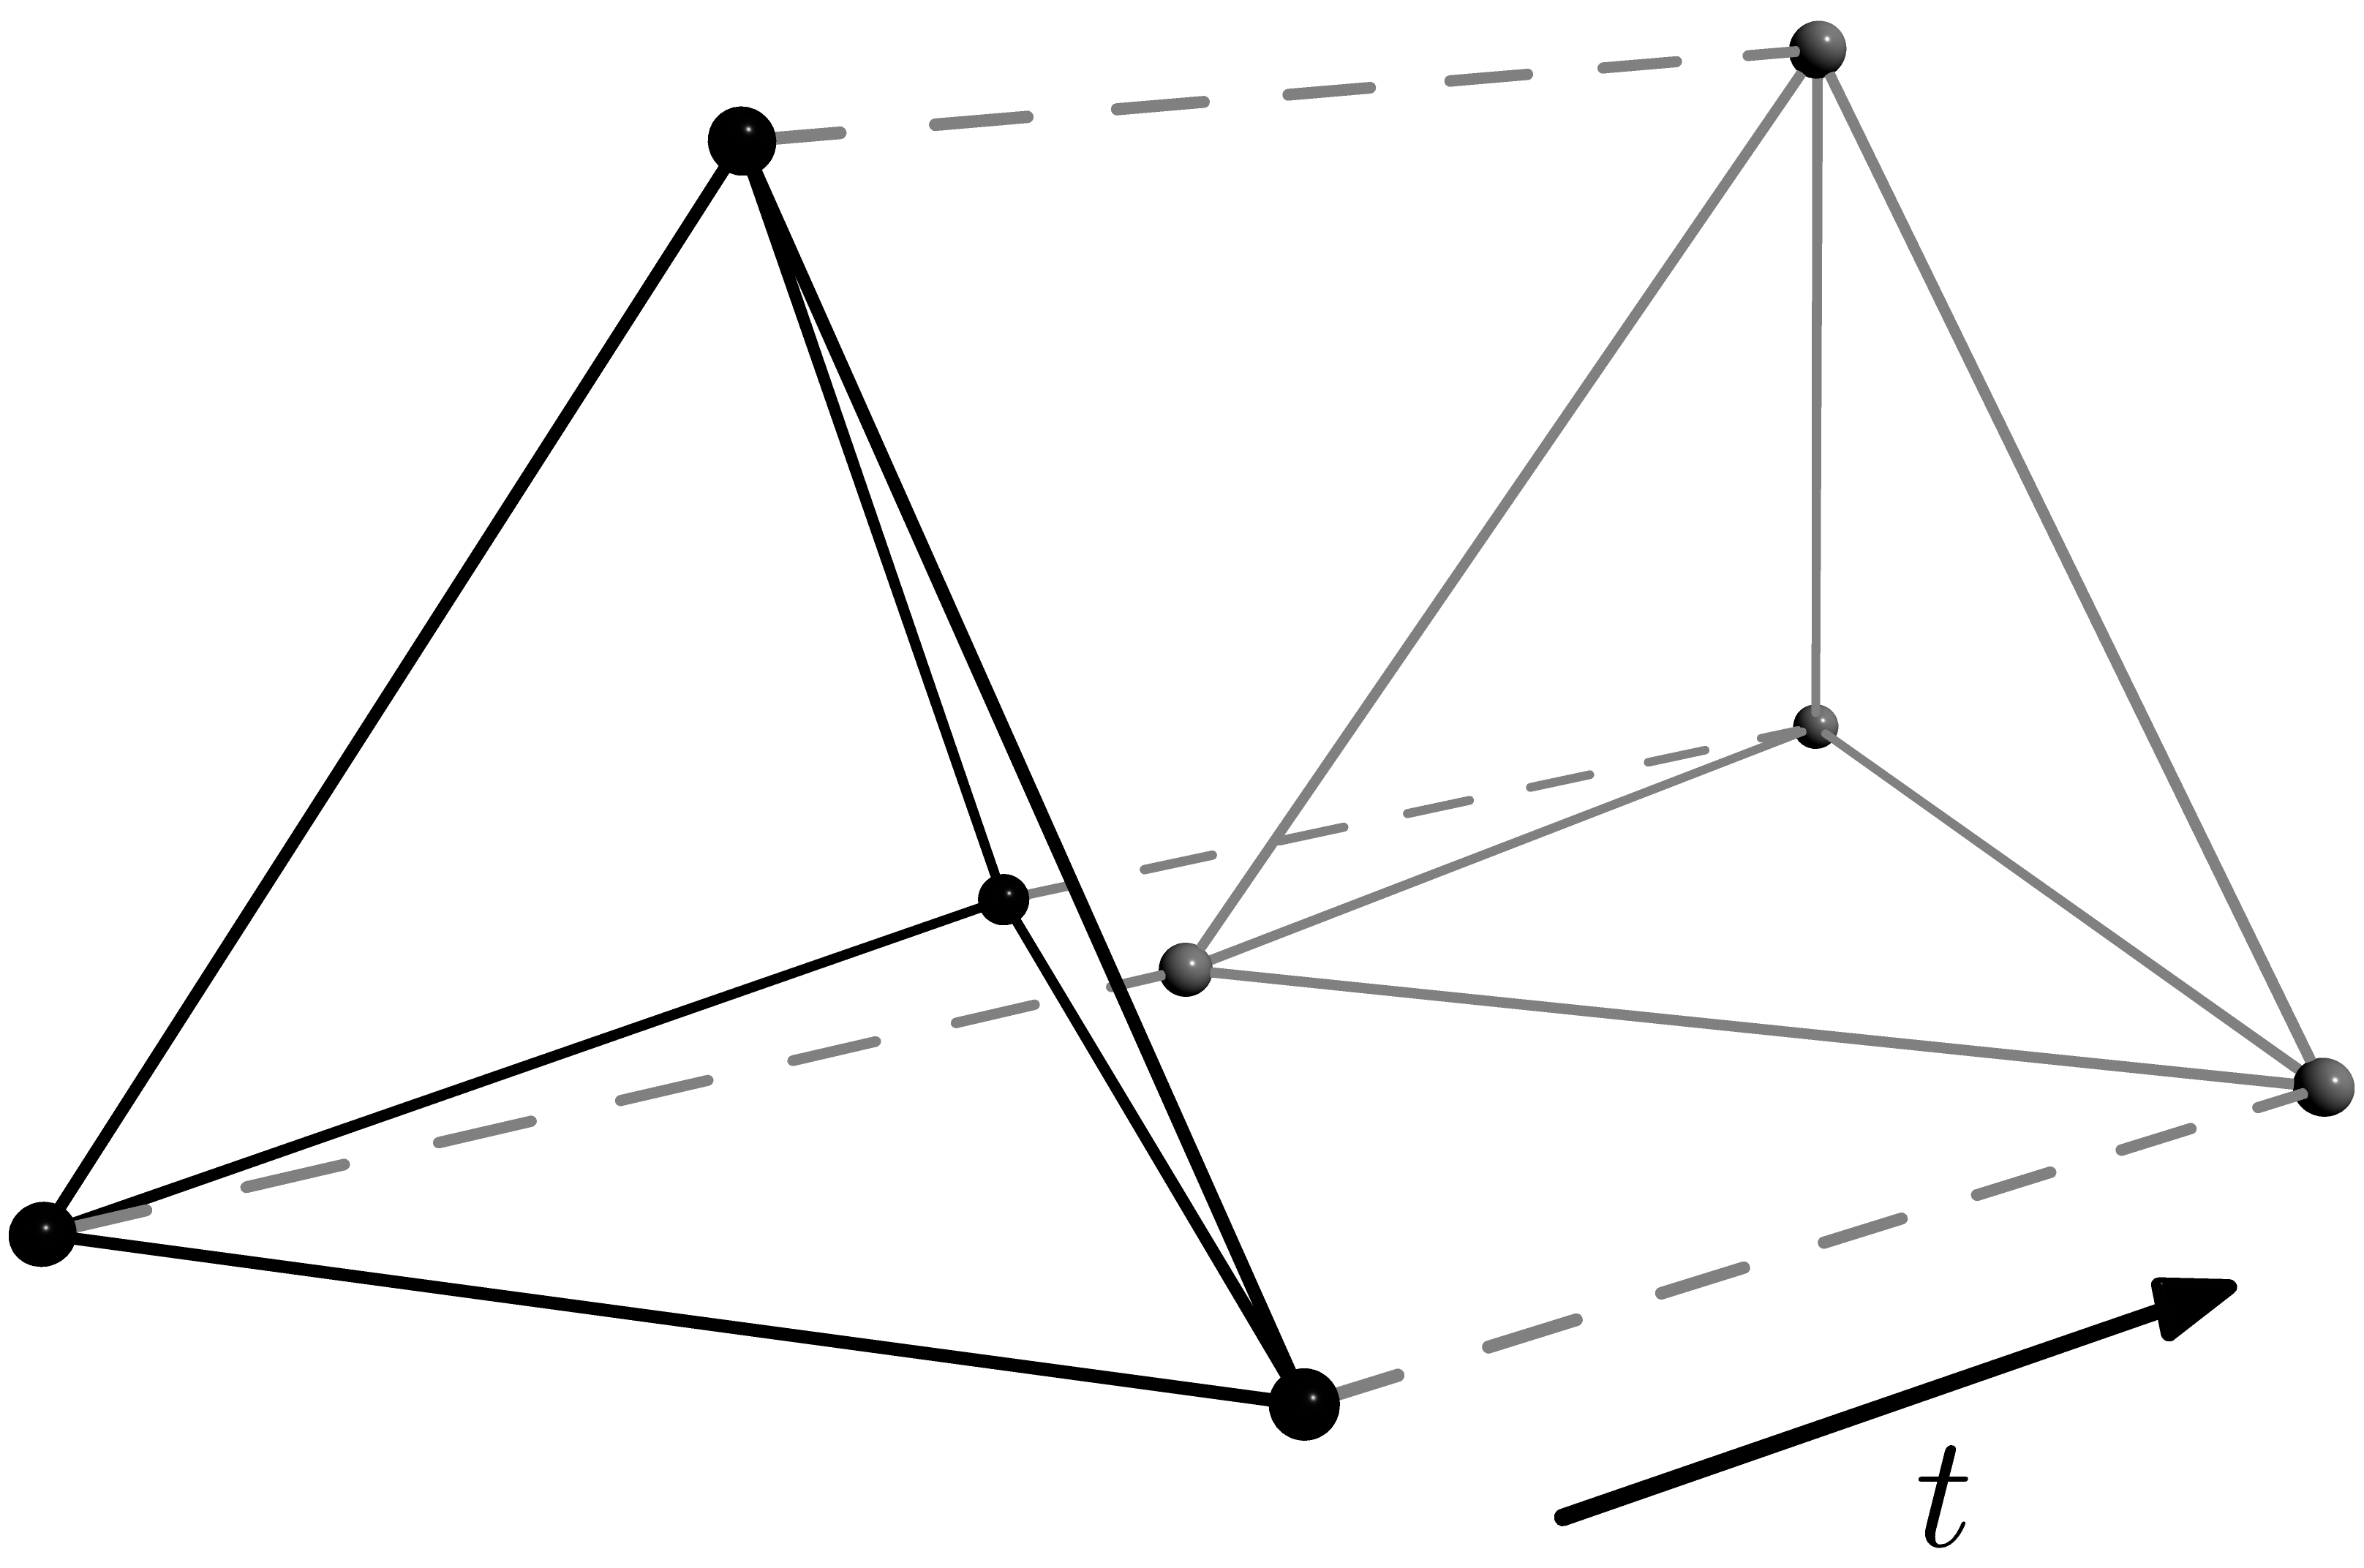
\includegraphics[width=0.4\textwidth]{figures/tetraprism_new.png}\label{fg:tet_domain}}
    \hspace{24pt}
    \subfloat[六面体柱积分域]{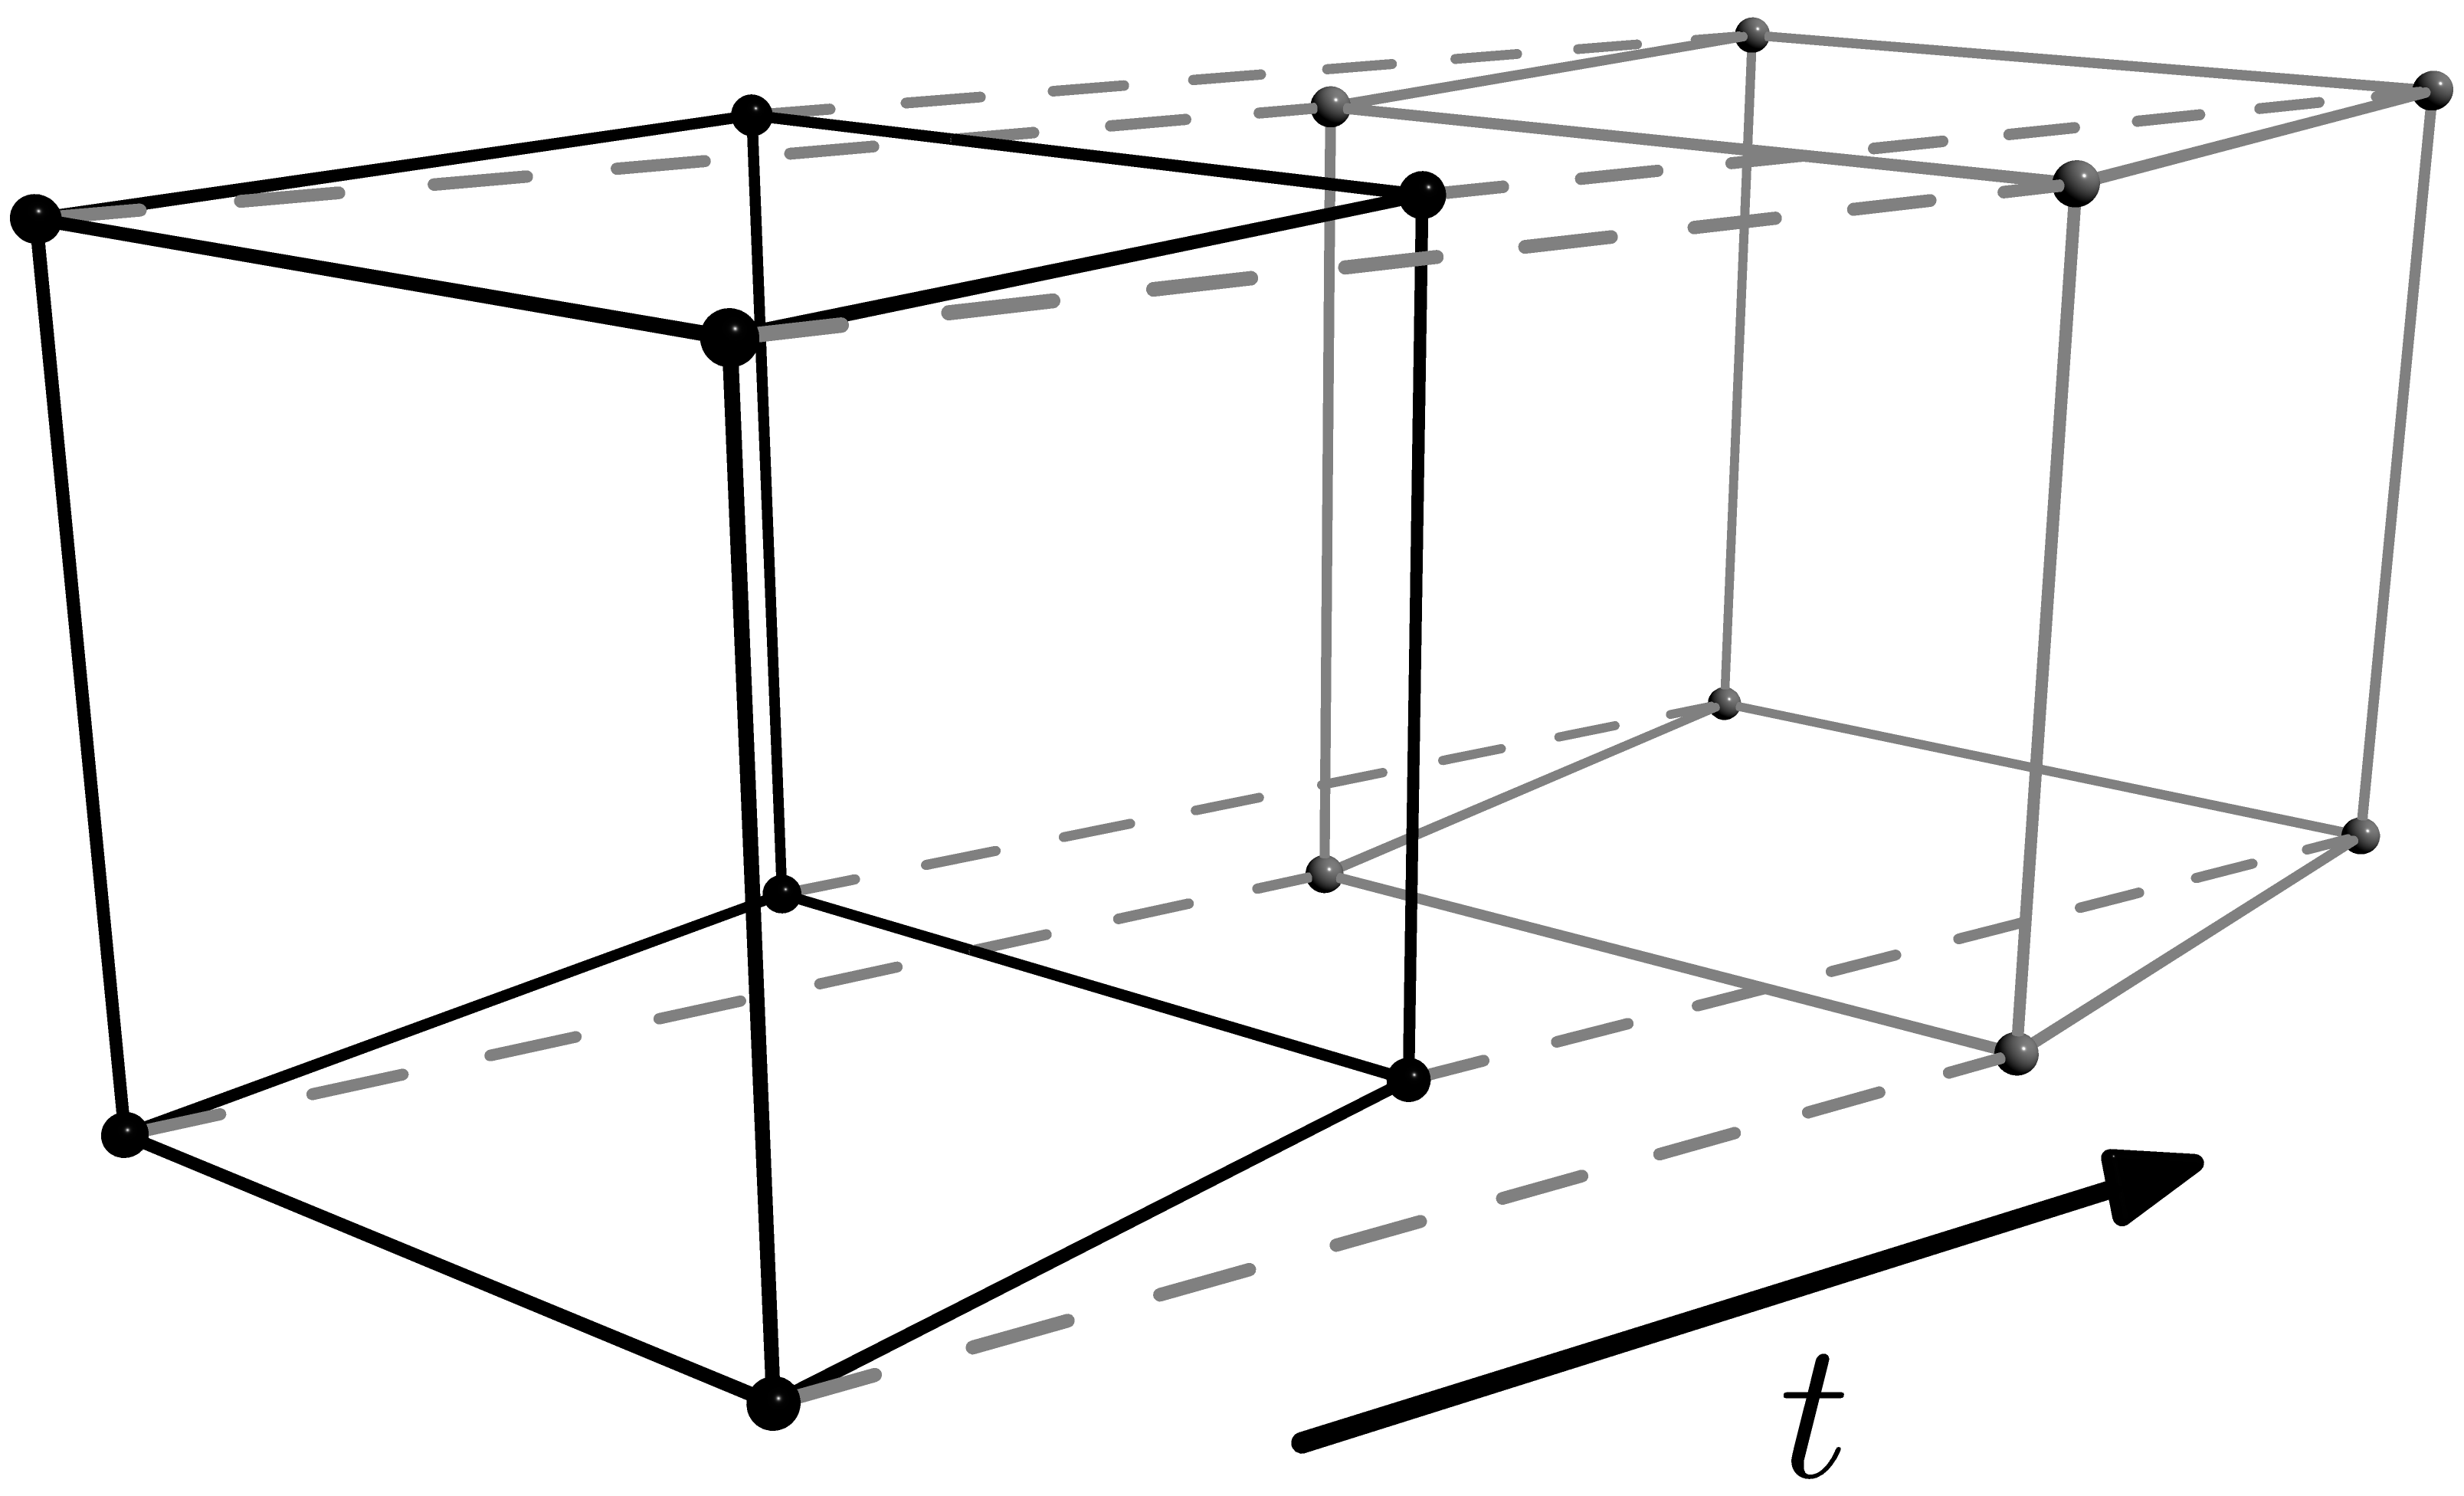
\includegraphics[width=0.4\textwidth]{figures/cubeprism_new.png}\label{fg:hex_domain}}
    \caption{四维空间背景积分域}
    \label{fg:domain}
\end{figure}

最后,通过分片试验验证所提数值积分方案是否满足变分一致性,同时利用典型波动问题测试其计算精度。

\subsubsection*{\bfseries (4)任意节点分布时空混合离散伽辽金无网格分析方法}
首先,将时空混合离散再生核无网格形函数及其光滑梯度引入拉格朗日乘子型伽辽金弱形式\eqref{eq:1}中,并采用优化的伽辽金无网格数值积分方案进行积分,得到相应的离散控制方程。
由式\eqref{eq:1} 可知,所提时空混合离散伽辽金弱形式中双线性算子均为同一算子,区别在于变量$u_h$和$p_h$所处的空间不一致。
造成空间不一致的原因在于$u_h$和$p_h$的本质边界条件不一致。当$u_h$和$p_h$采用相同的近似方式进行离散时,单独将施加本质边界条件部分的刚度矩阵分出,可得到如下所示离散控制方程:
\begin{equation}
    \begin{bmatrix} 
        \boldsymbol K + \boldsymbol K_{u} & \boldsymbol K \\
        \boldsymbol K & \boldsymbol K_{p} 
    \end{bmatrix} 
    \begin{Bmatrix}
        \boldsymbol u \\ \boldsymbol p
    \end{Bmatrix} =
    \begin{Bmatrix} \boldsymbol f_u \\ \boldsymbol f + \boldsymbol f_p \end{Bmatrix}
    \label{eq:3} 
\end{equation}
其中,$\boldsymbol K_u$和$\boldsymbol f_u$、$\boldsymbol K_p$和$\boldsymbol f_p$分别为施加与$u_h$和$p_h$相关的本质边界条件刚度矩阵和力向量。式\eqref{eq:3}中,刚度矩阵$\boldsymbol K$重复在三个地方使用,将利用该特点优化程序结构,降低内存开销。

同时,$u_h$与$p_h$的本质边界条件需要采用满足伽辽金法变分一致性的施加方案进行施加。本项目将在申请人所提基于Hellinger--Reissner原理伽辽金无网格本质边界条件施加方案的基础上,研究适用于拉格朗日乘子型时空混合离散伽辽金弱形式的变分一致型施加方案,确保全域的变分一致性。

随后,为进一步提升稳定性,将引入基于位移解梯度变化的自适应节点加密方案,对波的传播动态进行精确捕捉。同时,在求解离散控制方程时,拟嵌入基于Krylov子空间法的并行计算库,对程序进行提速。最后,通过典型波动问题和实际工程算例验证所提方法的有效性和可靠性。

\subsection{可行性分析}
针对制定的研究内容和研究目标,申请人对研究方案的每一部分进行项目的可行性分析,具体如下:

研究内容(1)拟基于拉格朗日乘子法建立适用于任意节点离散的时域末端虚位移本质边界条件。
该方案提供了一个全新的思路施加虚位移本质边界条件。
针对这部分研究内容的可行性,申请人采用一维杆结构动力问题对此研究方案进行初步验证。
不失一般性,问题的空间区域与时间区域所构成的二维时空区域采用均布的线性三角形有限元单元进行离散,图 \subref*{fg:bar_2} 为位移云图,从图中可以看出在均布节点的离散情况下,拉格朗日乘子型时空混合伽辽金弱形式无需分块网格技术,即可得到稳定的数值结果。
图 \subref*{fg:bar_3} 为该问题的位移云图和位移误差收敛率分析,从图中可以看出该混合离散框架可以保证理论误差收敛率。
但是,当时间区域节点间距过大时,数值色散问题将导致计算结果出现振荡现象,需要本项目后续研究内容的成果解决此问题。从拉压杆动力测试当中可以初步数值验证所提研究方案可行,后续可在此基础上,延续制定的研究方案逐步完善该方法的理论基础,达成所提研究目标。

\begin{figure}[!h]
    \centering 
    % \includegraphics[width=2cm]{figures/cubeprism.png}
    % \subcaptionbox{\includegraphics{figures/cubeprism.png}}
    \subfloat[问题模型与精确解]{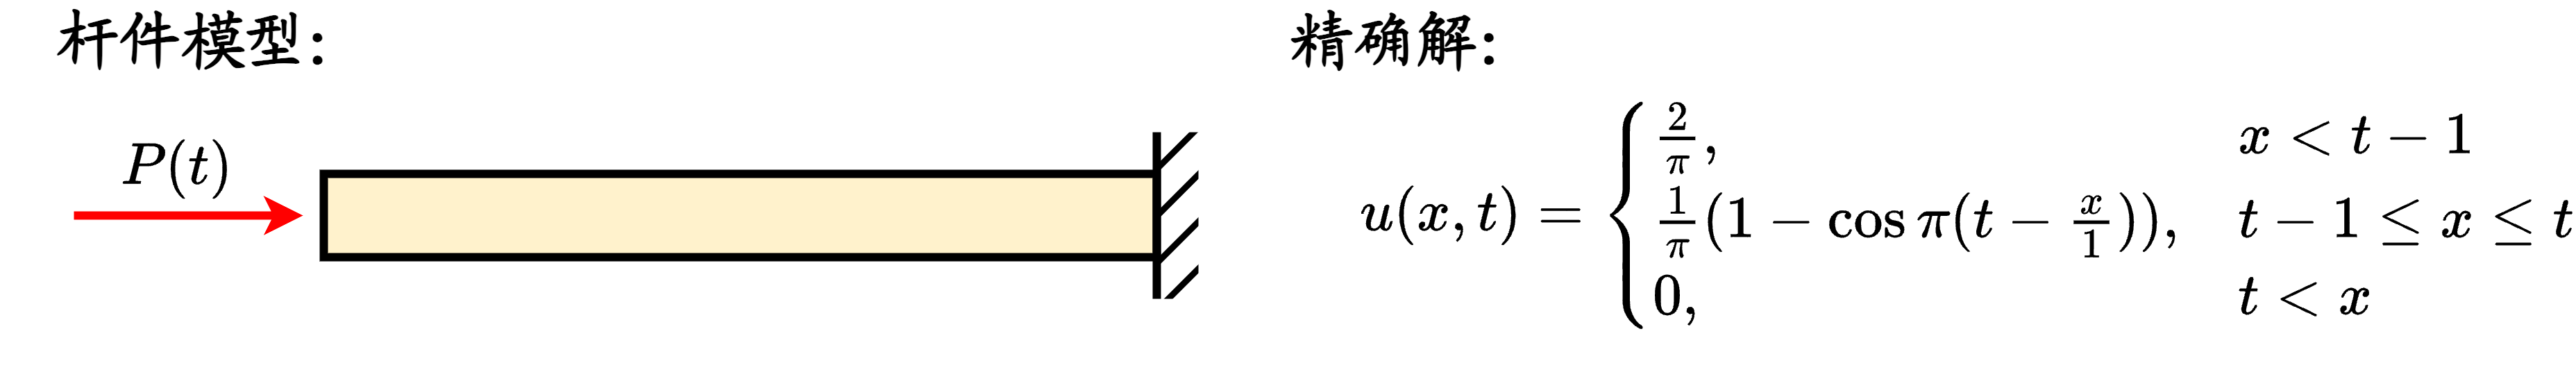
\includegraphics[width=\textwidth]{figures/bar.png}\label{fg:bar_1}}

    \subfloat[位移云图]{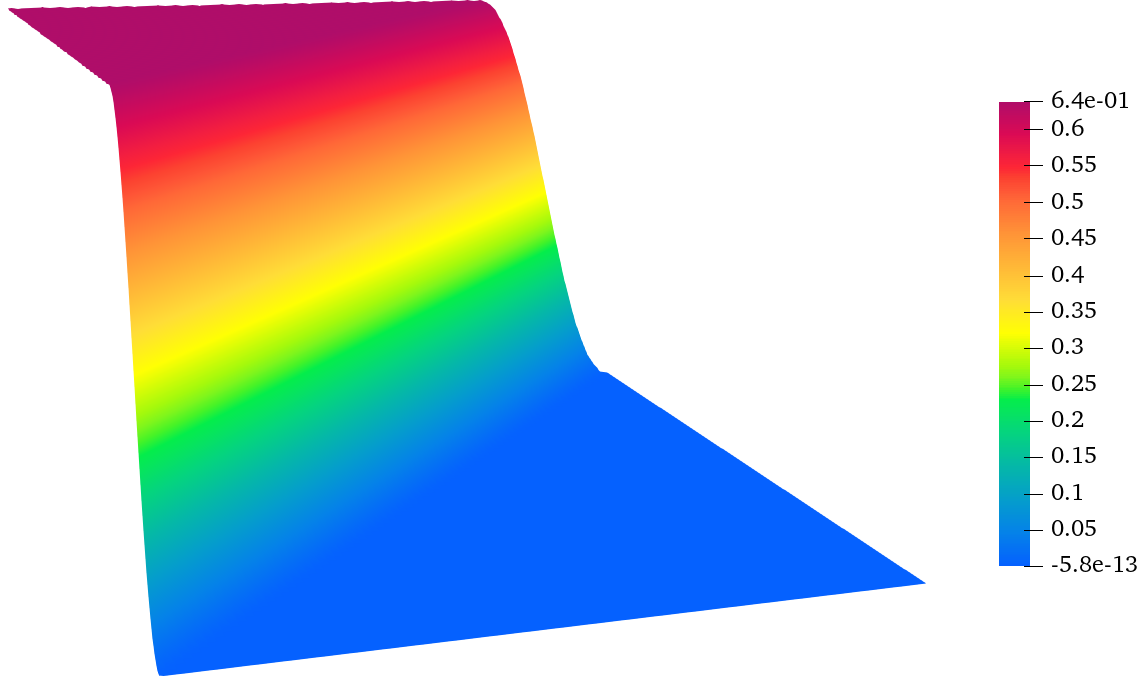
\includegraphics[width=0.50\textwidth]{figures/bar_contour.png}\label{fg:bar_2}}
    % \hspace{24pt}
    \subfloat[误差收敛率分析]{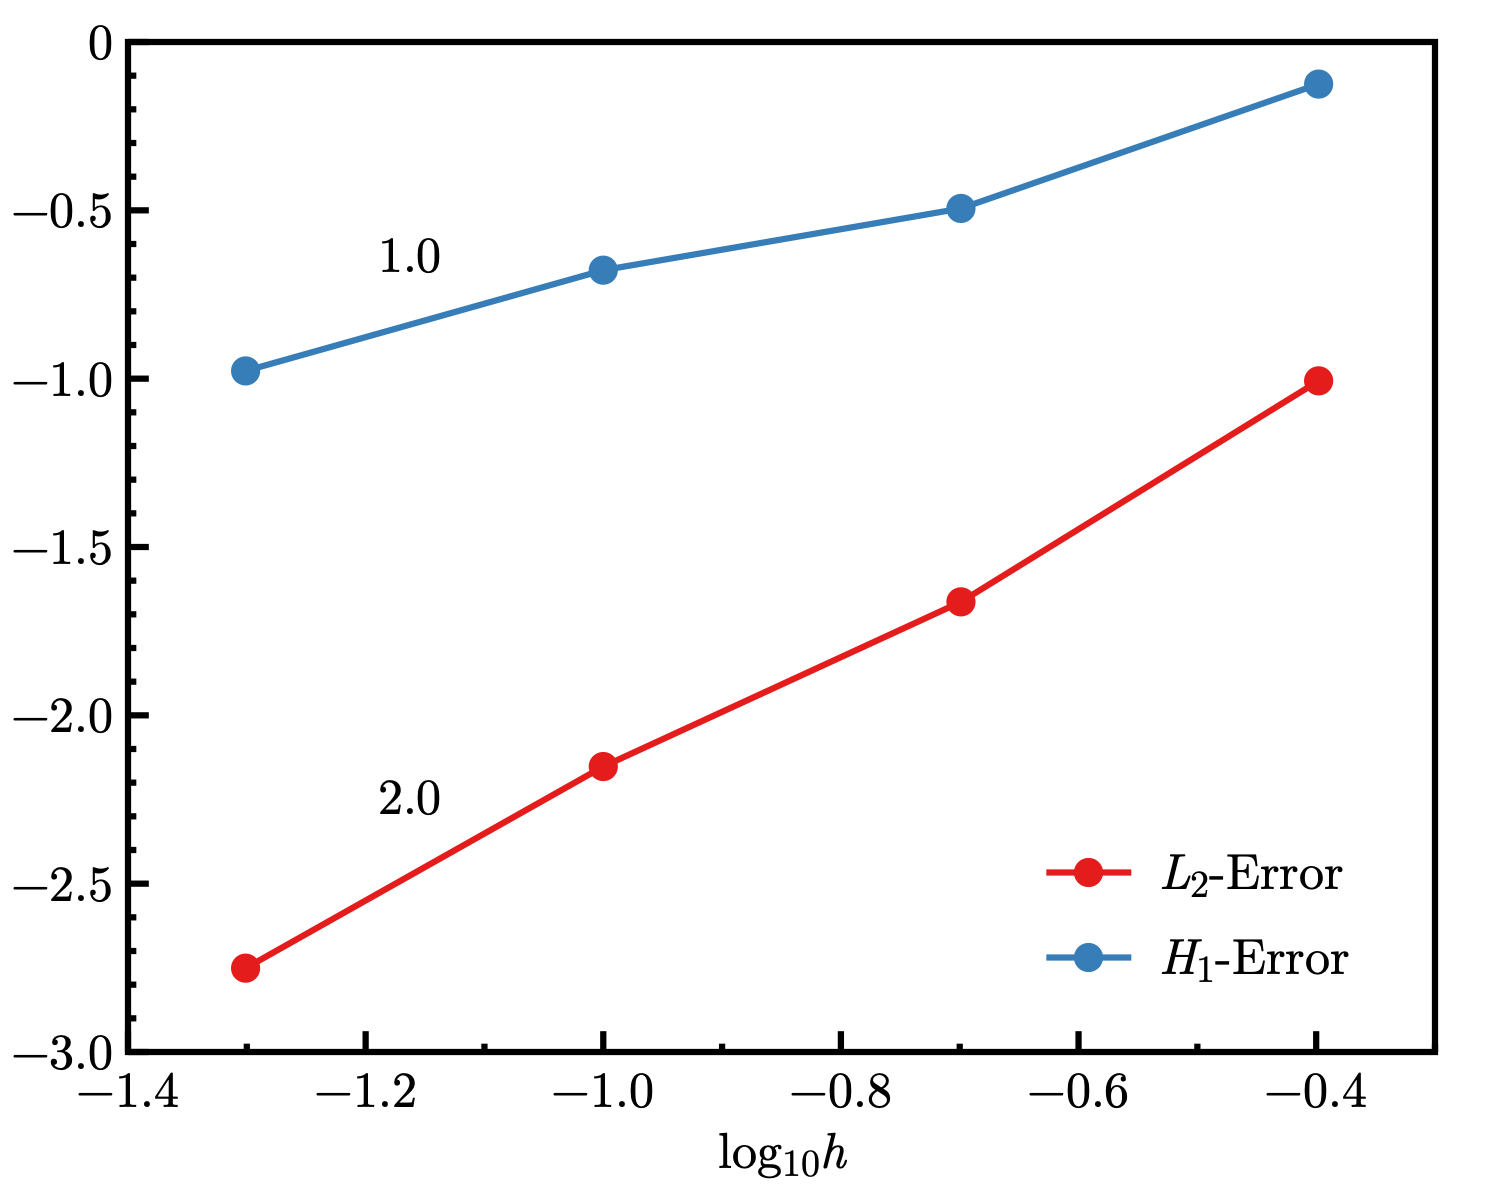
\includegraphics[width=0.50\textwidth]{figures/error.png}\label{fg:bar_3}}
    \caption{拉格朗日型虚位移边界条件施加方案初步测试:杆结构动力问题}
    \label{fg:bar}
\end{figure}

研究内容(2)拟建立可缓解数值色散现象的再生核无网格近似方案。
该方案通过对时空混合离散伽辽金法进行局部截断误差估计,确定时间域和空间域混合离散的近似阶次。
并利用再生核无网格近似,构造相对应阶次的时空混合离散形函数。
针对伽辽金无网格法误差分析方面,申请人已对伽辽金无网格法的正交性条件\cite{wu2021}和动力分析中的频率\cite{wu2018a}提出了相应的误差估计。
尤其是动力分析中的频率误差估计,建立该估计所采用的方法与本项目研究方案(2)中拟采用的方案一致,均为基于特征解的局部截断误差估计的方法,在一定程度上说明此研究方案可行。
在时空混合离散再生核近似方面,申请人在构造非常规基向量再生核近似形函数也具有一定的研究经验,
曾针对Helmholtz方程提出基于三角函数基向量的再生核近似\cite{wang2020b}。
而Helmholtz方程也是本项目研究波动问题稳态解的控制方程。
相关研究成果支持研究方案(2)可行。

研究内容(3)拟在时空混合离散伽辽金弱形式中引入再生光滑梯度无网格数值积分方案进行求解,并利用数值积分点在积分域间的共享特性优化全局积分点数,提升计算效率。
申请人针对高阶伽辽金无网格数值积分过程提出了嵌套子域积分法\cite{wang2016b}和再生光滑梯度积分法\cite{wang2019a},再生光滑梯度积分法也是本研究内容拟采用的方法。
该方法是基于假定应变理论变分一致型无网格数值积分方案的通用理论框架,适用于任意形式基向量的无网格形函数,如研究方案(2)所提时间域与空间域不同阶次的基函数。
在再生光滑梯度理论框架下,伽辽金无网格法采用与基函数阶次相对应的数值积分方案即可满足积分约束条件,保证计算精度。同时,该框架支持针对伽辽金弱形式中的背景积分域积分和边界积分优化积分点数量,提升计算效率。申请人与合作者还将该方法推广至相场断裂模型分析\cite{wu2020a}、Helmholtz问题分析\cite{wang2020b}、薄板壳问题\cite{wu2023,wu2024}、动力分析\cite{Fu2022}和应变梯度问题\cite{du2022},系列工作说明本研究内容具可行性。

研究内容(4)拟建立时空混合离散伽辽金无网格法,该方法需要结合研究内容(1--3)中所提的时域末端虚位移本质边界条件施加方案、时空混合离散再生核无网格近似方案、时空混合离散变分一致型伽辽金无网格数值积分方案,并引入基于位移解梯度变化的自适应节点加密方案和求解线性方程组的并行计算库,提升方法的精度和效率。
在该方法建立过程中,本质边界条件施加方案需进一步改进,使其满足变分一致性。
申请人基于Hellinger--Reissner和Hu--Washizu多变量变分原理提出了弹性力学、薄板和薄壳问题的变分一致型伽辽金无网格法本质边界条件施加方案\cite{Wu2022b,wu2023,wu2024}。
该方法不仅完备了再生光滑梯度积分法的理论基础,并且能保证整体伽辽金法的变分一致性,且无需额外稳定项和人工经验参数。
该方法也是本研究方案计划采用方法,相关研究成果支持本研究方案的可行性。
其次,基于位移解梯度变化的自适应节点加密方案和线性方程组并行求解方案都是较为成熟的技术方法,没有特别的技术障碍,不影响本研究内容的可行性。

综上所述,申请人就本项目的关键科学问题和研究方案中的关键步骤的相关内容进行了系列研究,取得了一定的研究成果,为本项目的研究提供了坚实的基础。鉴于以上分析,本项目所提的研究方案具有很强的可行性。

